%        File: main.tex
%     Created: Thu Oct 27 09:00 PM 2011 C
% Last Change: Thu Oct 27 09:00 PM 2011 C
%
\documentclass[a4paper,12pt]{book}

\usepackage[pdfpagelabels,draft,implicit=false]{hyperref}
\usepackage[utf8]{inputenc}
\usepackage[francais]{babel}
\usepackage{graphicx}
\usepackage{amsmath}
\usepackage[Sonny]{fncychap}
%\usepackage{fullpage}
\usepackage{setspace}
\usepackage{mathrsfs} %lettre ronde
\usepackage{multirow}
\usepackage{fancyhdr}
\pagestyle{plain}
\usepackage{pdfpages}


\setstretch{1.2}
\lhead{\nouppercase{\rightmark}}
\rhead{\nouppercase{\leftmark}}

\renewcommand{\sectionmark}[1]{}

\begin{document}

\frontmatter 

\author{Romain Vincent} 
\title{\Huge Détection d'un spin nucléaire unique à l'aide d'un transistor de spin} 
\date{Décembre 2012}
\maketitle
\thispagestyle{empty}
\sloppy %permet de forcer certains retours à la ligne plutôt qu'un mot qui dépasse

\tableofcontents

\mainmatter 

%\chapter*{Introduction}
\markboth{Introduction}{Introduction}
\addcontentsline{toc}{chapter}{Introduction}
\setcounter{figure}{0}

\section*{Motivations}
L'électronique a pris une place centrale dans la vie de tous les jours. Elle est impliquée dans le moindre de nos gestes : du simple micro-ondes au super calculateur nous donnant la météo de la semaine. A tel point qu'elle offre aujourd'hui un angle d'attaque nouveau jusque dans l'analyse de la société~(cf concept de fracture numérique). Cette place centrale oblige les acteurs de cette industrie à relever deux défis majeurs : fabriquer des composants moins chers et plus performants. Pendant longtemps la pierre angulaire de cette course à la performance a été la réduction de la taille des composants jusqu'à atteindre, à l'heure actuelle, des tailles caractéristiques de quelques dizaines de nanomètres. Mais ce paradigme du toujours plus petit a atteint ses limites et la technique impliquée dans la fabrication des dispositifs devrait bientôt marquer le pas. Les performances se gagnent désormais par l'implémentation de nouvelles architectures comme le prouve l'apparition, depuis quelques années déjà, de processeurs multi-coeurs, ou bien encore, par l'amélioration des systèmes d'exploitation afin de tirer parti, de manière efficace, de ces nouvelles architectures. Mais en aucun cas, les solutions proposées ne font appel à de nouveaux concepts de la physique ou bien encore de la chimie. Or, c'est bien de ces deux disciplines que pourraient venir les prochaines évolutions majeures de l'électronique.

La chimie, tout d'abord, étudie depuis longtemps déjà les phénomènes d'auto-organisation. Ce terme traduit la tendance qu'ont certaines molécules à s'organiser de façon à former des structures complexes, sans intervention extérieure. Cette capacité à l'auto-organisation pourrait être utilisée dans l'avenir pour fabriquer, sans l'usage de techniques lithographiques, des composants micro-électroniques organiques. Ceci est d'autant plus vraisemblable que la chimie organique sait désormais synthétiser des composés conducteurs ou semi-conducteurs, déjà mis en œuvre dans des composants conventionnels tels que les transistors à films fins organiques. Mais l'électronique moléculaire, pour être une candidate sérieuse, doit également offrir la possibilité de fabriquer des composants de spintronique, c'est-à-dire, des composants sensibles au spin des électrons. A l'heure actuelle, ces composants sont au centre des technologies les plus courantes, tels que les disques durs ou bien encore les mémoires magnétiques~(MRAM en anglais). La chimie dispose pour cela de molécules possédant des propriétés magnétiques particulières : les aimants moléculaires. Ces derniers pourraient, par exemple, \^etre utilisés pour la fabrication d'électrodes ferromagnétiques organiques, ou bien encore, dans l'implémentation de vannes de spin.

Mais changer les méthodes de fabrication n'est qu'une partie de la solution. Il est également possible d'utiliser les nouveaux concepts issus de la mécanique quantique, comme le montre les résultats d'une discipline relativement récente : l'information quantique. Cette dernière a notamment des implications dans deux domaines de l'informatique moderne : la recherche dans les bases de données~(à l'aide de l’algorithme de Grover) et la cryptographie~(grâce à l'algorithme de Shor mais également de par les propriétés des observables en mécanique quantique). Les bases de données sont au centre de nombreuses applications et ont à faire face à un nombre toujours plus grand d'informations à traiter. Pour prendre l'exemple du moteur de recherche Google, celui-ci doit traiter les informations extraites de 30 trillions de documents, et ce, à raison de 40000 requêtes par seconde~(chiffres de Google en 2012). Et ces chiffres sont en constante hausse et nécessitent donc une puissance de calcul croissante. Une alternative à cette course à la puissance pourrait être trouvée dans la fabrication d'ordinateurs quantiques qui, grace à l'algorithme de Grover, pourraient réduire non seulement la puissance nécessaire mais également la mémoire utilisée. De m\^eme, face à la croissance des flux de données, mais aussi de la cybercriminalité, il est devenu primordial de mettre en place des solutions de cryptage efficaces. C'est à cette t\^ache que se sont attelés les spécialistes de ce que l’on appelle la cryptographie quantique. Le concept de réduction du paquet d'onde, par exemple, pourrait jouer un rôle central dans la détection d'interception, par un tiers, d'un signal envoyé.

Pour rendre cette révolution possible, il faut pouvoir stocker et manipuler les données à l'aide de bits quantiques ou qbits. De nombreux objets physiques peuvent implémenter ces fameux qbits au sein des laboratoires, mais lorsque l'on songe à une application à plus grande échelle, la liste des candidats diminue de façon significative. Les aimants moléculaires sont des prétendants sérieux à la fabrication de cette nouvelle électronique. Comme nous le détaillerons dans la suite, ils peuvent faire l'objet d'une approche ``\textit{Bottom-Up}", c'est-à-dire, s'appuyant sur l'auto-organisation de la matière. En outre, ils possèdent un moment magnétique dont l'orientation permettrait de coder l'information binaire, comme c'est déjà le cas dans les disques durs par exemple. Enfin, les aimants moléculaires constituent des systèmes quantiques susceptibles d'\^etre manipulés et pourraient donc \^etre utilisés en tant que qbits.

Les travaux que nous allons présenter dans la suite tentent de répondre aux problématiques que nous venons d'évoquer en montrant qu'une spintronique moléculaire est possible. Cette dernière permettrait d'utiliser les molécules aimants comme des qbits en utilisant non seulement le moment magnétique électronique comme support de l'information, mais également le spin nucléaire. Cette dernière possibilité rend les aimants moléculaires d'autant plus attractifs que le spin nucléaire a été présenté comme composant de base idéal à l'informatique quantique~\cite{Kane1998}.

\newpage
 
\section*{Plan de thèse}

Nous commencerons, dans le premier chapitre, par dresser un rapide aperçu de la spintronique et de l'électronique organique, soulignant les problématiques inhérentes à  chacun de ces domaines. Nous discuterons ensuite du magnétisme moléculaire et des synergies possible avec l'électronique, aboutissant à la spintronique moléculaire. Nous continuerons par une brève histoire de l'électronique moléculaire avec la réalisation du premier transistor à molécule, puis nous présenterons les évolutions ayant conduit à la réalisation du premier dispositif de spintronique moléculaire à l'échelle d'une molécule unique. Enfin, nous retracerons les évolutions de cette thématique au sein de notre groupe pour conclure en évoquant les tous derniers résultats obtenus.

Dans une deuxième partie, nous décrirons les techniques de fabrication nous permettant d'obtenir un transistor à molécule unique. Nous insisterons tout d'abord sur la nécessité de disposer d'une bonne grille, en soulignant les critères importants et les techniques de fabrication permettant de les remplir. Nous détaillerons ensuite la fabrication des nanofils d'or ainsi que la technique d'électromigration permettant d'obtenir nos nano-cassures. Nous terminerons par une brève présentation de notre technique de dépôt de molécules et une description succincte de la première caractérisation électrique.

Enfin dans le dernier chapitre, nous exposerons l'ensemble de nos résultats expérimentaux. Nous détaillerons dans un premier temps ce qui fait du terbium un candidat idéal aux applications de spintronique moléculaire et nous décrirons ses principales propriétés magnétiques. Nous analyserons ensuite les différents mécanismes susceptibles de coupler le transport électronique au magnétisme moléculaire, en envisageant deux configurations : l'une directe et l'autre indirecte. Puis nous nous intéresserons aux propriétés électroniques de notre transistor. En particulier, nous extrairons de cette analyse l'intensité et la nature de l'interaction entre les électrons donnant naissance au courant mesuré et le moment magnétique moléculaire. Ensuite, nous analyserons plus finement les sauts de conductance différentielle associés au retournement de l'aimantation. Nous détaillerons tout d'abord notre procédure de détection et d'analyse des sauts de conductance. Nous montrerons qu'ils permettent, par une analyse de leur position en champ magnétique, de mesurer indirectement l’état du spin nucléaire du terbium. En outre, nous utiliserons l'hystérésis en conductance induite par le couplage magnéto-transport pour identifier les différents axes de notre molécule aimant. Puis nous nous intéresserons au magnétisme électronique de l'aimant moléculaire TbPc$_{2}$ en insistant sur le rôle central du champ transverse dans nos mesures. Enfin, nous analyserons en détail la dynamique du magnétisme nucléaire. En particulier, nous mettrons en évidence un temps de vie des états nucléaires de près de dix secondes, ainsi que l'aspect non-destructif de notre technique de mesure. Nous démontrerons également que cette dynamique est fortement influencée par l'environnement électrostatique de notre système. De plus, part une analyse des populations nucléaires nous mettrons en évidence la bonne thermalisation de ce dernier malgré le courant électrique traversant notre transistor.
%\chapter{Spintronique moléculaire}

\section{Spintronique et Électronique moléculaire}
La micro-électronique a su évoluer au gré des développements scientifiques. Elle a tout d'abord su tirer avantage des travaux sur la magnéto-résistance géante au travers d'une nouvelle discipline : la spintronique. Pendant presque deux décennies, celle-ci a permis d'améliorer de plusieurs ordres grandeurs les capacités de stockage des composants électroniques. Plus récemment, le développement de molécules organiques semi-conductrices~\cite{Tsumura1986,Horowitz1990,Lin1997} a poussé encore une fois l'électronique dans une nouvelle voie, celle de l'électronique moléculaire.

Ces deux évolutions pourraient bientôt fusionner pour tirer avantage des concepts issues de la spintronique et du formidable potentiel de l'électronique moléculaire.

\subsection{La spintronique}
La spintronique est une branche de l'électronique où, en plus de la charge, le degré de liberté du spin de l'électron est utilisé. Elle est notamment à l'origine des avancés technologiques les plus récentes telles que la MRAM~(Magnetic Random Access Memory) ou bien encore les têtes de lecture des disques durs~(cf Fig.\ref{SpinValve}.\textbf{b}). Mais le dispositif le plus célèbre, à la base des technologies précédemment citées, reste sans doute la vanne de spin. Celui-ci permet de filtrer les électrons en fonction de l'orientation de leur spin (soit \textit{up}, soit \textit{down}), autorisant un couplage direct entre magnétisme et courant électrique. La découverte du phénomène de magnétorésistance géante~(cf Fig.\ref{SpinValve}.\textbf{a}), à l'origine de ce filtrage, a d'ailleurs value à ses découvreurs, Albert Fert~\cite{Baibich1988} et Peter Grünberg~\cite{Gruenberg1986}, le prix Nobel de Physique en 2007.

\begin{figure}
\centering \includegraphics[scale=0.45]{Spintronique/SpinValve/SpinValve.pdf}
\caption{\textbf{a} : mesure de la résistance d'une valve de spin mettant en évidence la magnéto-résistance géante~(extrait de ~\cite{Baibich1988}).  \textbf{b} : Schéma d'une tête de lecture de disque dur dont le fonctionnement est basé sur le phénomène de magnéto-résistance~(extrait de~\cite{Hitoshi2001}).}
\label{SpinValve}
\end{figure}



La spintronique, dans ses applications, reste cependant cantonnée au stockage de  l'information~\cite{Awschalom2007}. Des propositions de transistors de spin, directement commandés par le spin électronique, ont pourtant été faites~\cite{Datta1990}, et certains dispositifs ont également été réalisés~\cite{Johnson1996,Huang2007}. Mais de tels systèmes n'ont pas, pour l'instant, quitté les laboratoires.

De plus, elle se heurte aux défis de la miniaturisation, qui ne lui sont pas spécifiques, mais qui se posent à l'ensemble de l'électronique. Le salut des futurs dispositif pourrait bien se trouver dans l'électronique organique.

\subsection{L'électronique organique}
Devant le besoin toujours plus grand de miniaturisation des dispositifs, les chercheurs et les industriels se sont vite rendus compte des limites des techniques de fabrication traditionnelles. Elles consistent à partir d'un matériau massif, et de graver en son sein, les structures nanométriques nécessaires à la production de l'électronique actuelle. C'est l'approche dite``\textit{Top-Down}"

Devant les progrès récents de la chimie organique, une seconde solution est apparue, faisant appel à cette dernière  pour produire les objets de petite taille et les disposer de manière contrôlée : c'est l'approche dite ``\textit{Bottom-Up}". Dans cette approche, deux caractéristiques des molécules sont exploités : leur capacité à s'auto-assembler, c'est à dire à adopté une configuration précise ``programmée" à travers les ligands; la possibilité de fabriquer des milliards de molécules toutes identiques, avec une grande pureté. 

L'histoire de l'électronique moléculaire est cependant relativement récente. Comme le rappelle G. Horowitz dans~\cite{Klauk2007}, l'industrie s'est finalement intéressée à ce domaine de l'électronique lorsque les semi-conducteurs organiques sont devenus plus performants, en terme de mobilité électronique, que le silicium amorphe~\cite{Lin1997}.
\begin{figure}
\centering \includegraphics[scale=0.45]{Spintronique/MolecularElec/MolecularElec.pdf}
\caption{\textbf{a} : Photographie d'un substrat de polymide contenant des transistors organiques. \textbf{b} : Vue en coupe d'un transistor organique~(figure extraite de~\cite{Sekitani2010}).}
\label{MolecularElec}
\end{figure}


Depuis, de nombreux dispositifs issus de l'électronique moléculaire ont vu le jour, comme les  transistors à base de films fins organiques (ou OFTFs - cf Fig.\ref{MolecularElec}). Mais aucune application n'a, à ce jour, tiré partie de la taille nanométrique des molécules, et la route est encore longue avant l'obtention de dispositifs commerciaux ne mettant en jeux que quelques molécules, voire une seule.

Comme le rappelle les auteurs de~\cite{Gatteschi2006} , une conséquence plus inattendue du développement de l'électronique moléculaire est d'avoir participé à l'essor du magnétisme moléculaire, domaine que nous allons aborder maintenant.


\section{Le magnétisme moléculaire}
Essayer de dresser un panel complet du magnétisme moléculaire est un travail complexe auquel je ne m'attacherai pas ici. Pour cela, je renvois le lecteur à~\cite{Gatteschi2006} et son excellente introduction. Je ne vais souligner ici que quelques étapes présentant certains des phénomènes physiques majeurs mis en évidence dans les aimants moléculaires.

\begin{figure}
\centering \includegraphics[scale=0.45]{Spintronique/MolecularMag/MolecularMag.pdf}
\caption{\textbf{a} : Première mesure du phénomène de QTM sur un cristal moléculaire de Mn$_{12}$Ac~(extrait de~\cite{Thomas1996}). \textbf{b} : Mise en évidence du phénomène d'interférence relatif au retournement de l'aimantation d'un cristal moléculaire de Fe$_{8}$~(extrait de~\cite{Wernsdorfer1999}).}
\label{MolecularMag}
\end{figure}

La première mesure d'un effet quantique sur un aimant moléculaire~(SMM ou Single Molecular Magnet) a été obtenue en 1995 à partir d'un échantillon de poudre d'une molécule maintenant bien connue : le Mn$_{12}$Ac~\cite{Friedman1996}. Quelques temps plus tard, cette mesure était confirmée à l'aide d'un cristal moléculaire de Mn$_{12}$Ac~\cite{Thomas1996}. Cet effet quantique est connu sous le nom de retournement de l'aimantation par effet tunnel~(ou QTM - Quantum Tunneling of the Magnetization).

Celui-ci correspond au retournement de l'aimantation d'une molécule malgré la présence d'une barrière de potentiel entre les deux orientations opposées. Tout ce passe comme si l'aimantation passait à travers cette barrière par effet tunnel, d'où le nom. Ceci n'est possible que lorsque deux états du système, situés de part et d'autre du puits de potentiel, sont amenés en résonance à l'aide d'un champ magnétique. Le phénomène de QTM ne peut se faire que pour des valeurs de champ magnétique bien précises donnant lieux à des mesure de cycle d'hystérésis présentant des marches~(cf Fig.\ref{MolecularMag}.\textbf{a}). L'annexe concernant les aimants moléculaires traite en détail de ce phénomène.

Trois ans plus tard, Wolfgang Wernsdorfer et Roberta Sessoli mettaient en évidence l'oscillation des \textit{splitings} tunnels dû à un effet quantique d'interférence semblable à la phase de Berry~\cite{Wernsdorfer1999}~(cf Fig.\ref{MolecularMag}.\textbf{b}). Dans ce phénomène, les interférences se font entre le différents ``chemins" que l’aimantation peut prendre sur la sphère de Bloch lors de son renversement. Ceci se traduit par une variation dans les probabilités de retournement et donc, par une modulation de la hauteur des marches associés au QTM.

La structure hyperfine de certains terres rares a pu également être explorée. En effet, la position en champ des retournements par QTM peut être, dans certains cas, fortement influencé par l'état du spin nucléaire. Le TbPc$_{2}$, où Terbium Double-Decker~( en référence aux avions à deux ailes), a notamment été caractérisé en détail à l'aide de la technique microSQUID, et les paramètres de couplage hyperfin ont pu être extraits de la mesure de l'aimantation d'un cristal moléculaire~\cite{Ishikawa2005}. D'autre noyaux que le Tb ont également été analysés avec succès à l'aide d'une structure moléculaire identique~\cite{Ishikawa2005a}.

\begin{figure}
\centering \includegraphics[scale=0.45]{Spintronique/MolecularMag2/MolecularMag2.pdf}
\caption{\textbf{a} : Structure du \textit{cluster} de Fe$_4$. \textbf{b} : Représentation des différent mode d'ancrage~(extrait de~\cite{Mannini2010}).}
\label{MolecularMag2}
\end{figure}

Mais les progrès de l'électronique moléculaire n'ont pas laissé la communauté du magnétisme indifférente et la question de l'interaction entre aimant moléculaire et surface métallique à commencé à se poser. Une étude portant sur une molécule de Mn$_{12}$ déposée sur une surface d'or a été réalisée en 2008~\cite{Mannini2008} en combinant différents moyens d'analyse~(XAS et XMCD). Elle conclue que la structure de l'aimant moléculaire est modifiée lorsque ce dernier est déposé sur une surface et que le magnétisme est également affecté. Cette fragilité des aimants moléculaire a été confirmée par une seconde série de mesure~\cite{Mannini2009} soulignant l'importance du choix du SMM pour les applications de spintronique moléculaire.

Plus récemment, l'équipe de Roberta Sessoli a mis en évidence le retournement de l'aimantation de molécule de Fe$_{4}$ ancrée à l'aide de ligand sur une surface d'or~\cite{Mannini2010}~(cf Fig.\ref{MolecularMag2}). De plus, ils ont pu montrer qu'il était possible de contrôler la direction préférentielle de l'aimantation adopté par les SMM une fois sur la surface, par le choix de ligands adaptés.

Cependant, une meilleure compréhension du magnétisme moléculaire et de ses interactions avec l’environnement passe par le développement de la spintronique moléculaire, seul moyen d'investigation à l'échelle de la molécule unique. C'est donc également dans cette voie que se sont engagé à la fois les chimiste et les physiciens comme nous allons le voir maintenant.


\section{La spintronique moléculaire}
La spintronique moléculaire a pour but de combiner les techniques de la spintronique avec les nouveaux développements de l'électronique moléculaire et de la chimie, afin de produire de nouveaux dispositifs susceptibles de compléter ou éventuellement remplacer les technologies tout semi-conducteurs déjà existantes. Cette discipline a connu une évolution rapide ces dernières années, bénéficiant des dernières avancés en matière de lithographie, mais aussi de la mise en synergie du travail des physiciens et des chimistes. 

Dans ce paragraphe, je ne présenterai bien sûr qu'une petite partie des nombreux travaux effectués dans le domaine. Ceci ne constitue donc en aucun cas une liste exhaustive des expériences réalisées, ni m\^eme une sélection des travaux les plus importants. Elle permettra, je l'espère, au lecteur de situer nos recherches par rapport à celles en cours dans d'autres laboratoires. De plus, je me limiterai ici aux dispositifs ne comportant qu'un nombre limité de molécules, de l'ordre de l'unité, généralement utilisés dans les laboratoires de recherche fondamentale.
\subsection{État de l'art}

\subsubsection*{Du premier transistor moléculaire...}
La première expérience de mesure de courant à travers une molécule unique a été faite en 1995 à l'aide un microscope à effet tunnel~\cite{Joachim1995}~( ou STM). Il s'agissait de mesurer la résistance à travers une molécule de C$_{60}$ déposée sur une surface d'or. Il n'était pas question d'obtenir un transistor, puisque seul deux terminaux étaient présents à savoir, la surface conductrice et la pointe du STM.

Cette expérience, et celles qui ont suivi, ont encouragé le développement de nouvelles techniques permettant de piéger une molécule unique dans un dispositif de mesure. C'est ainsi qu'est apparu la technique dite de``break junction"~\cite{Zhou1995}. Elle consiste à suspendre un fin pont métallique puis à plier le support jusqu'à obtenir une cassure. La taille de celle-ci peut être ensuite modulée en faisant varier la courbure imposée à l'échantillon. A l'aide de ce dispositif, Reed et ses collègues ont pu mesurer, en 1997, des molécules de benzene-1,4-dithiol et montrer l'influence du couplage entre les électrodes et la molécule, sur la conductance mesurée~\cite{Reed1997}. Cette technique présente cependant l'inconvénient de ne pas pouvoir disposer d'une grille permettant de moduler le potentiel de la molécule.

\begin{figure}
\centering 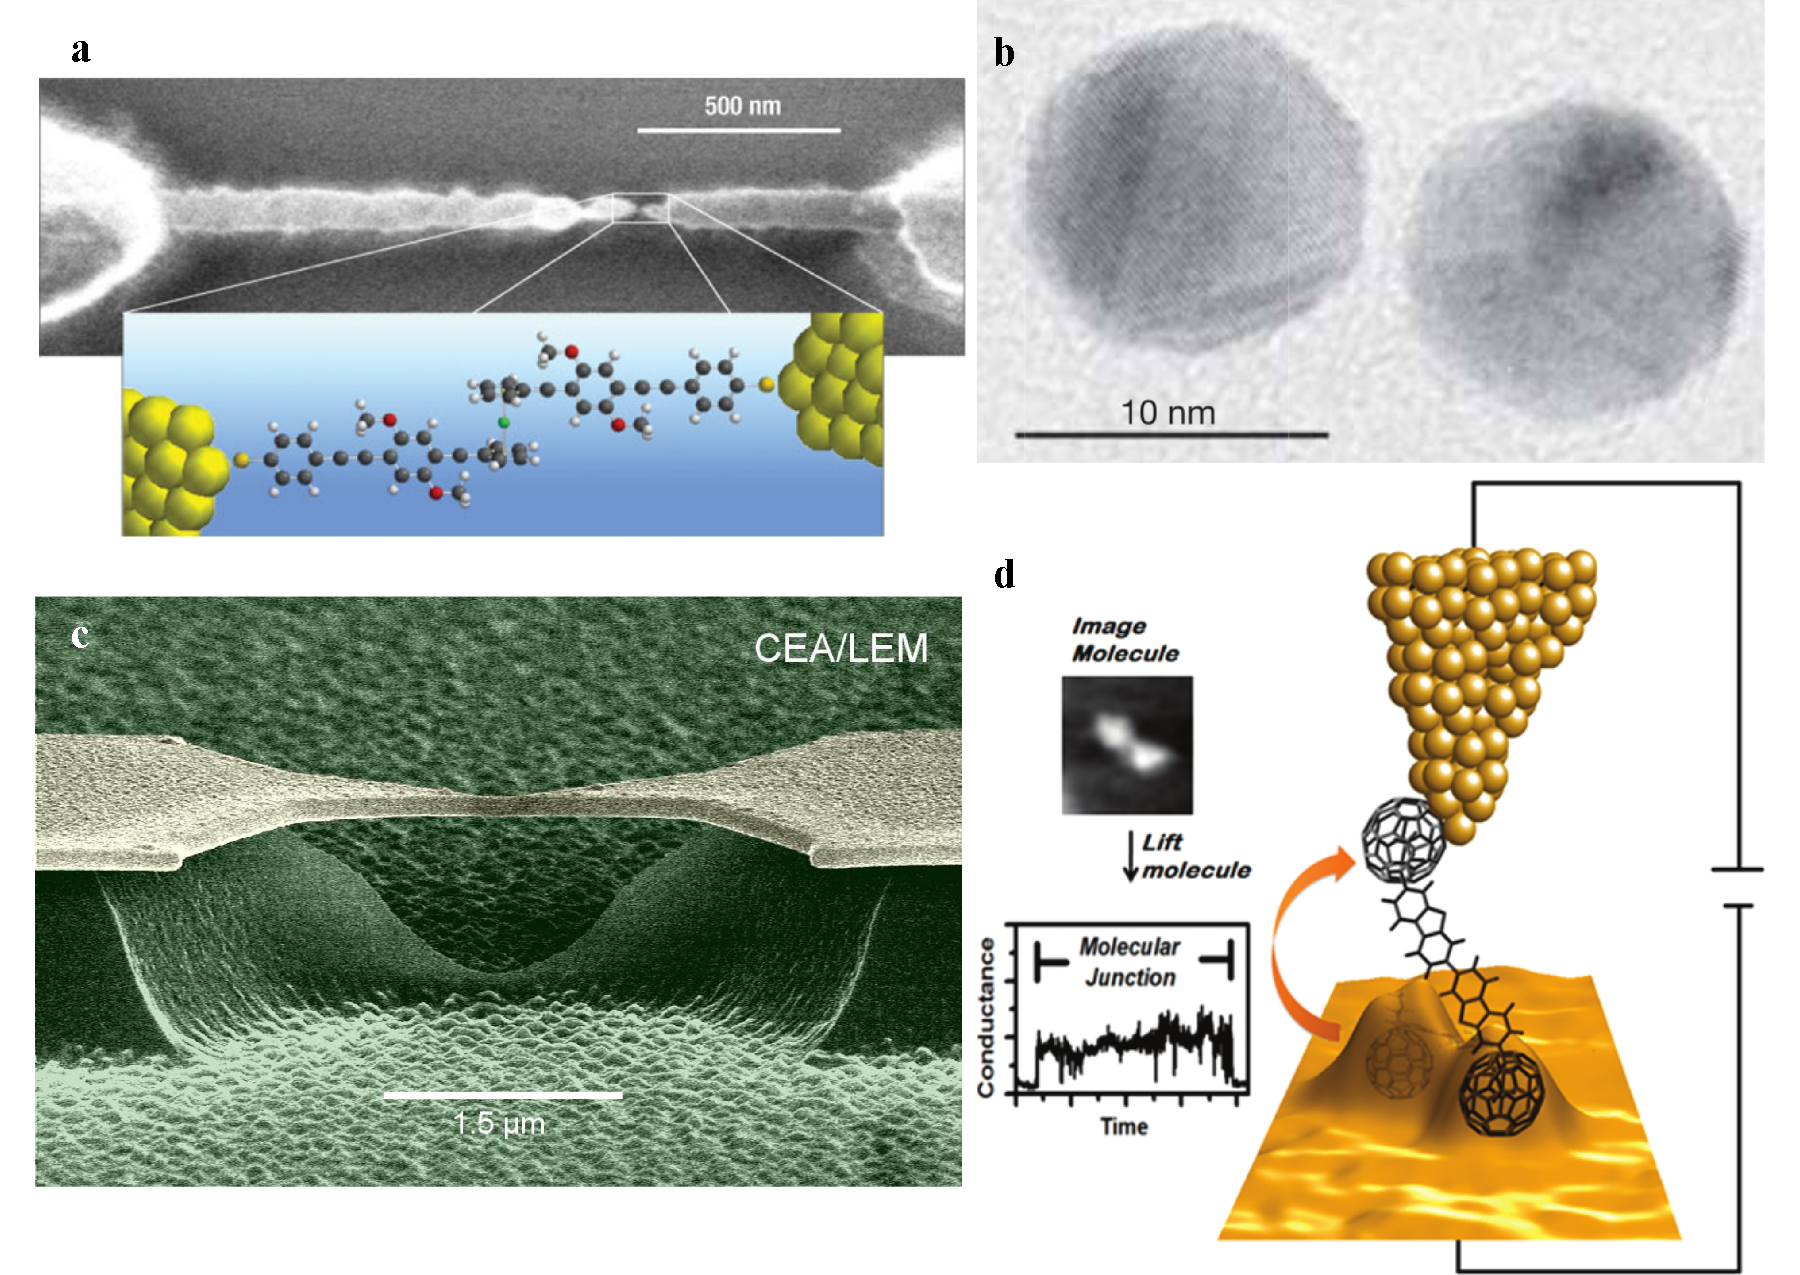
\includegraphics[scale=0.45]{Spintronique/MolSpintro2/MolSpintro2.pdf}
\caption{\textbf{a} : Structure de trois molecules : 1,4-benzenedimethanethiol~(BDMT), 4,4'-biphenyldithiol~(BPD) et bis-(4-mercaptophenyl)-ether~(BPE). \textbf{b} : Mécanisme de prise de contact. \textbf{c-e} : Image par microscopie électronique à transmission~(TEM) des structure de dimer, trimer et tetramer composé de bille d'or de $50\,nm$. \textbf{f} : image TEM d'un dimer à base de BDMT constitué par deux billes d'or de $10\,nm$. Le nanomètre qui sépare les deux billes correspond approximativement à la taille de la molécule de BDMT~($0.9\,nm$).Figure extraite de~\cite{Dadosh2005}}
\label{MolSpintro2}
\end{figure}


Pour pallier à cet inconvénient, il a fallu attendre encore 3 ans et la réalisation du premier transistor à molécule unique~\cite{Park2000}. Celui-ci consistait en un atome de C$_{60}$ piégé entre deux électrodes d'or et une grille. Ce dispositif a été obtenue en faisant circuler une forte densité de courant dans un fil fin d'or, venant provoquer la migration des atomes au niveau du point faible et provocant une cassure de l'ordre du nanomètre. Le phénomène d'électromigration est un phénomène bien connu des micro-électroniciens puisqu'il est à l'origine de certaines défaillances dans les puces et autres dispositifs électroniques~\cite{Ho1989,Tu1992}. Il a d'ailleurs donné son nom à la technique : l'électromigration. Nous présenterons cette dernière plus en détail dans le chapitre consacré à la fabrication de notre échantillon.

L'expérience menée sur ce premier transistor moléculaire avait pu mettre en évidence le couplage entre les vibrations moléculaires et la résistance du dispositif. De plus, la grille se révélait suffisamment efficace pour modifier l'état de charge de la molécule de C$_{60}$ permettant ainsi d'obtenir les premiers diamants de Coulomb associé à une molécule unique.

Une étape supplémentaire a été franchie par le groupe de A. Yacoby~\cite{Dadosh2005}~(cf Fig.\ref{MolSpintro2}) Ils ont mis au point la première approche réellement ``Bottom-Up" en attachant chimiquement une molécule à deux billes d'or de quelques nanomètres, pour venir ensuite contacter ces dernières à l'aide de deux électrodes.\`A ma connaissance, cette technique n'a pas été réutilisée depuis. Elle illustre néanmoins le rôle central que pourrait jouer la fonctionnalisation, dans une approche entièrement ``Bottom-Up"..

Cependant, dans ces dispositifs, aucune propriété propre aux molécules n'est utilisée et le seul spin en jeu dans les phénomènes observés reste celui de l'électron. Hors, l'avantage principal des molécules, outre leur taille, provient des différentes propriétés, notamment magnétique, que la chimie moderne peut leur conférer.

\subsubsection*{\`A la spintronique moléculaire}

L'année 2006 a vu paraître les deux premières expériences visant à insérer des aimants moléculaires au sein d'un gap afin d'obtenir les premiers dispositifs de spintronique moléculaire~\cite{Heersche2006,Jo2006}~(cf Fig.\ref{MolSpintro}). La première a été publiée par le groupe de H.S.J van der Zant et la seconde par le groupe de D.C. Ralph, et portaient toutes deux sur l'étude d'un aimant moléculaire bien connu : le Mn$_{12}$. Un des aspects intéressant de ces expériences, outre le magnétisme de la molécule, est la fonctionnalisation de cette dernière à l'aide de groupe thiol, afin de favoriser le couplage avec les électrodes d'or. Il illustre, encore une fois, la souplesse de la chimie et la possibilité qu'elle offre de fabriquer des molécules faites sur mesure, afin de faciliter certaines configurations ou certains comportements~(ici une forte affinité avec l'or).  

Cependant, les mesures en transport, bien que montrant une dépendance en champ magnétique complexe et des signes de conductance différentielle négative, n'ont pas permis de confirmer, de façon certaine, s'il s'agissait bien d'une molécule de Mn$_{12}$, ni même de savoir si les propriétés magnétiques de cette dernière avait été conservées durant la fabrication. Le groupe de D.C. Ralph conclue d'ailleurs ses travaux par la phrase suivante : ``\textit{We find significant variations between devices, indicating that the sample fabrication process and the device environment may affect our molecules}".

La première expérience réellement convaincante de transistors moléculaires mettant en jeu une molécule magnétique a été réalisée en 2008 dans le groupe de D.C. Ralph~\cite{Grose2008}. Toujours avec la technique d'électromigration, son équipe avait produit un transistor à base de N@C$_{60}$. Elle avait alors pu mettre en évidence, à travers des mesures en transport, le magnétisme lié à l'atome d'azote de spin S=3/2,  et remonter au couplage entre ce dernier et les électrons de la cage de C$_{60}$. 

\begin{figure}
\centering \includegraphics[scale=0.45]{Spintronique/MolSpintro/MolSpintro.pdf}
\caption{\textbf{a} : Structure du Mn$_{12}$ entouré de ligands thiols favorisant l'ancrage. \textbf{b} : Représentation schématique de la molécule de Mn$_{12}$ piégée entre les électrodes. \textbf{c} : Image de la jonctions obtenue par microscopie électronique. Le trait blanc correspond à $200\,nm$.~(extrait de~\cite{Heersche2006}).}
\label{MolSpintro}
\end{figure}

Il s'agit, à mes yeux, du premier dispositif que l'on peut qualifier de spintronique moléculaire à l'échelle de la molécule unique. En effet, les propriétés magnétiques de la molécule isolée se retrouvent de façon non-équivoque dans les mesures en transport. Ce n'est d'ailleurs pas surprenant car, fort de leur expérience avec le Mn$_{12}$, les auteurs avaient choisi le N@C$_{60}$ pour la robustesse de sa structure et de ses propriétés magnétiques, comme ils le précisent dans leur papier. 

Cependant, bien qu'ayant un moment magnétique, cette dernière n'appartient pas à la catégorie des aimants moléculaires. En effet, elle ne possède pas d'axe facile et l'orientation de son moment magnétique n'est déterminé que par le champ magnétique. Il est donc impossible d'observer dans cette molécule, les phénomènes quantiques présentés dans le cadre du magnétisme moléculaire.

Loin d'\^etre des échecs, ces différents travaux ont fournis un apport important au reste de la communauté notamment concernant les critères essentiels que doivent remplir les aimants moléculaires susceptibles d'être étudiés par les techniques expérimentales actuelles. Je détaillerai ces différents critères lorsque j'introduirai le Terbium double-Decker.
 
\subsection{La spintronique dans notre groupe}
Le groupe au sein duquel j'ai effectué ma thèse a une culture ancrée dans le nano-magnétisme et le magnétisme moléculaire. Une bonne partie des efforts de la fin des année 1990 et du début des années 2000 a été consacré à l'analyse et la caractérisation de systèmes magnétiques allant de la nanoparticule au cristal moléculaire  et plus récemment, l'aimant moléculaire isolé et le spin nucléaire unique. A chaque échelle de mesure correspond un appareil de mesure, et assez logiquement, plus le système à mesurer est petit, plus le détecteur l'est. Cette tendance est bien représentée dans la Fig.\ref{Group1}. Pour des particules macroscopiques, l'usage d'un SQUID est suffisant. Lorsque l'on veut caractérisé des particules de l'ordre de quelques dizaines de nanomètre ou bien encore un cristal moléculaire, l'usage d'un détecteur aussi sensible qu'un microSQUID est indispensable.


\begin{figure}
\centering \includegraphics[scale=0.45]{Spintronique/Group1/Group1.pdf}
\caption{\'Evolution des détecteurs en fonction de la taille de l'objet à mesurer.}
\label{Group1}
\end{figure}



Lorsque l'objet a détecter devient très petit, comme une molécule par exemple, il n'est plus vraiment possible de faire la distinction entre le détecteur et l'objet à mesurer. Il faut alors songer à fabriquer un dispositif électronique dont le fonctionnement même est influencé par le magnétisme de l'un de ses composants. Autrement dit, il faut faire appel à la spintronique et plus précisément, lorsque l'on s'intéresse aux molécules, à la spintronique moléculaire.

C'est dans ce cadre que se sont effectué les premiers travaux conduisant à la fabrication du premier nanosquid en 2006~\cite{CleuziouJ.-P.2006}. Celui-ci,  composé de deux liens faible supraconducteur à base de nanotube, a permis de mesurer, en transport, une astroide de Stoner–Wohlfarth~\cite{Cleuziou2011}, mesure caractéristique des propriétés magnétiques d'une nanoparticule. Ces dernières avaient pour particularité d'être insérées dans les Nanotube plutôt que déposées sur le dispositif, faisant parti intégrante du système de détection.

\begin{figure}
\centering 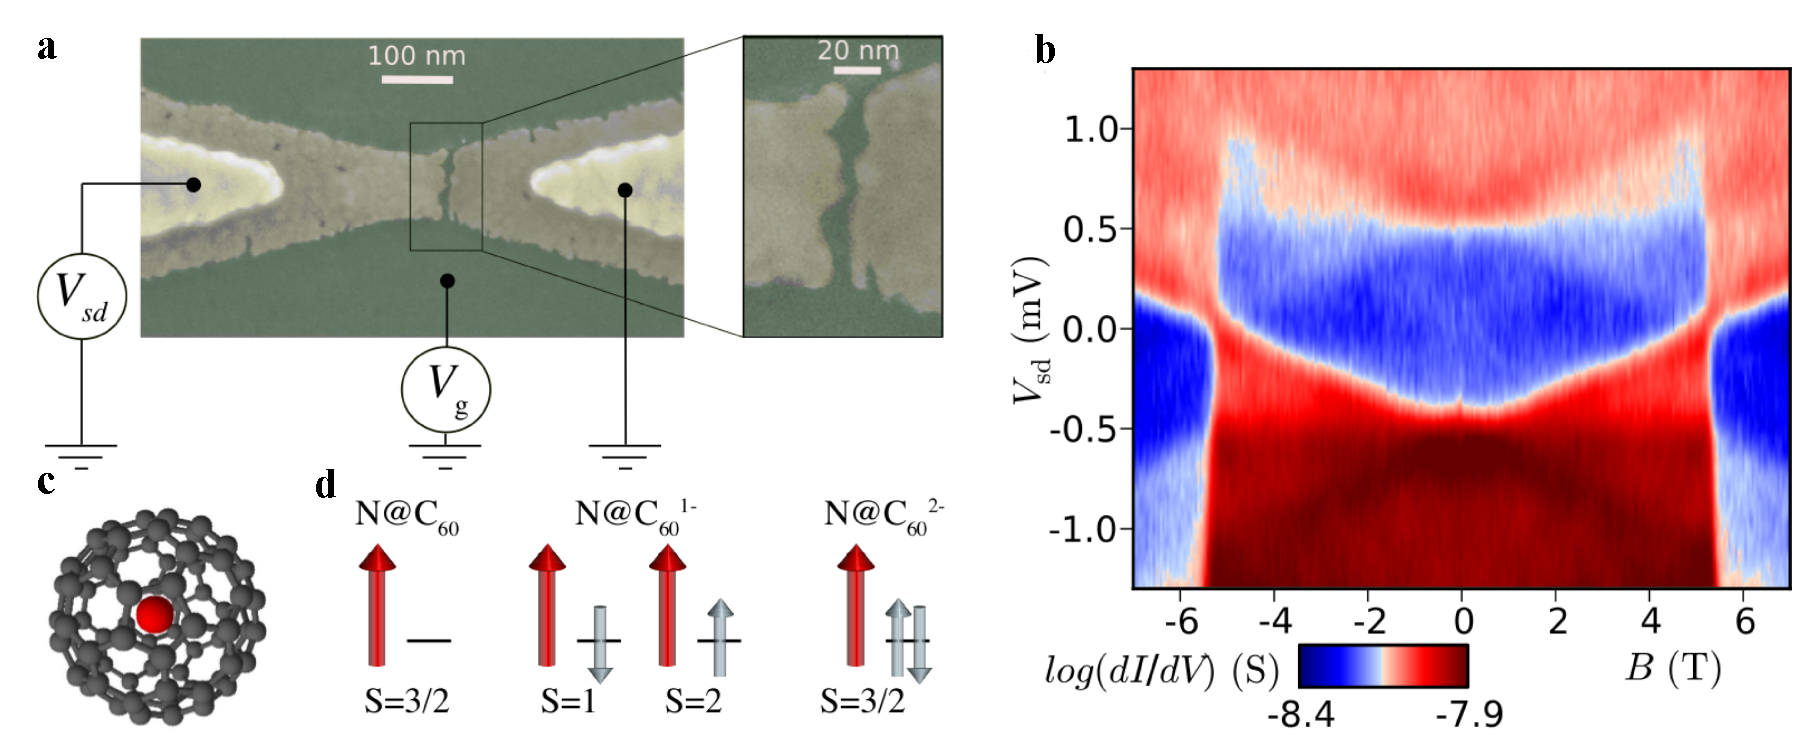
\includegraphics[scale=0.45]{Spintronique/RochC60/RochC60.pdf}
\caption{\textbf{a} : Image de microscope à force atomique montrant le fil d'or déposé sur une grille d'alumine. \textbf{b} : carte de conductance différentielle de l'échantillon en fonction de la tension soure-drain $V_b$ et la tension de grille $V_g$.}
\label{RochC60}
\end{figure}


Parallèlement aux travaux sur le nanoSQUID, notre groupe a développé, à partir des travaux de H. Park~\cite{Park1999}, sa propre technique d'électromigration basée sur une boucle de contre-réaction rapide. Ces travaux ont d'abord permis la réalisation d'un transistor moléculaire à base de C$_{60}$. Celui-ci à conduit à l'observation de nombreux phénomènes quantiques tels que l'effet Kondo sous-écranté~\cite{Roch2009} ou bien encore la transition de phase quantique~\cite{Roch2008}. Puis, en collaboration avec W. Harneit, nous avons étudié la molécule de N@C$_{60}$~\cite{Roch2011}, confirmant les résultats obtenus quelques temps plus tôt par D.C. Raplh et complétant ses observations par des mesures en cotunneling. L'ensemble de ces travaux peut être trouvé dans la thèse de Nicolas Roch.

\begin{figure}[H]
\centering 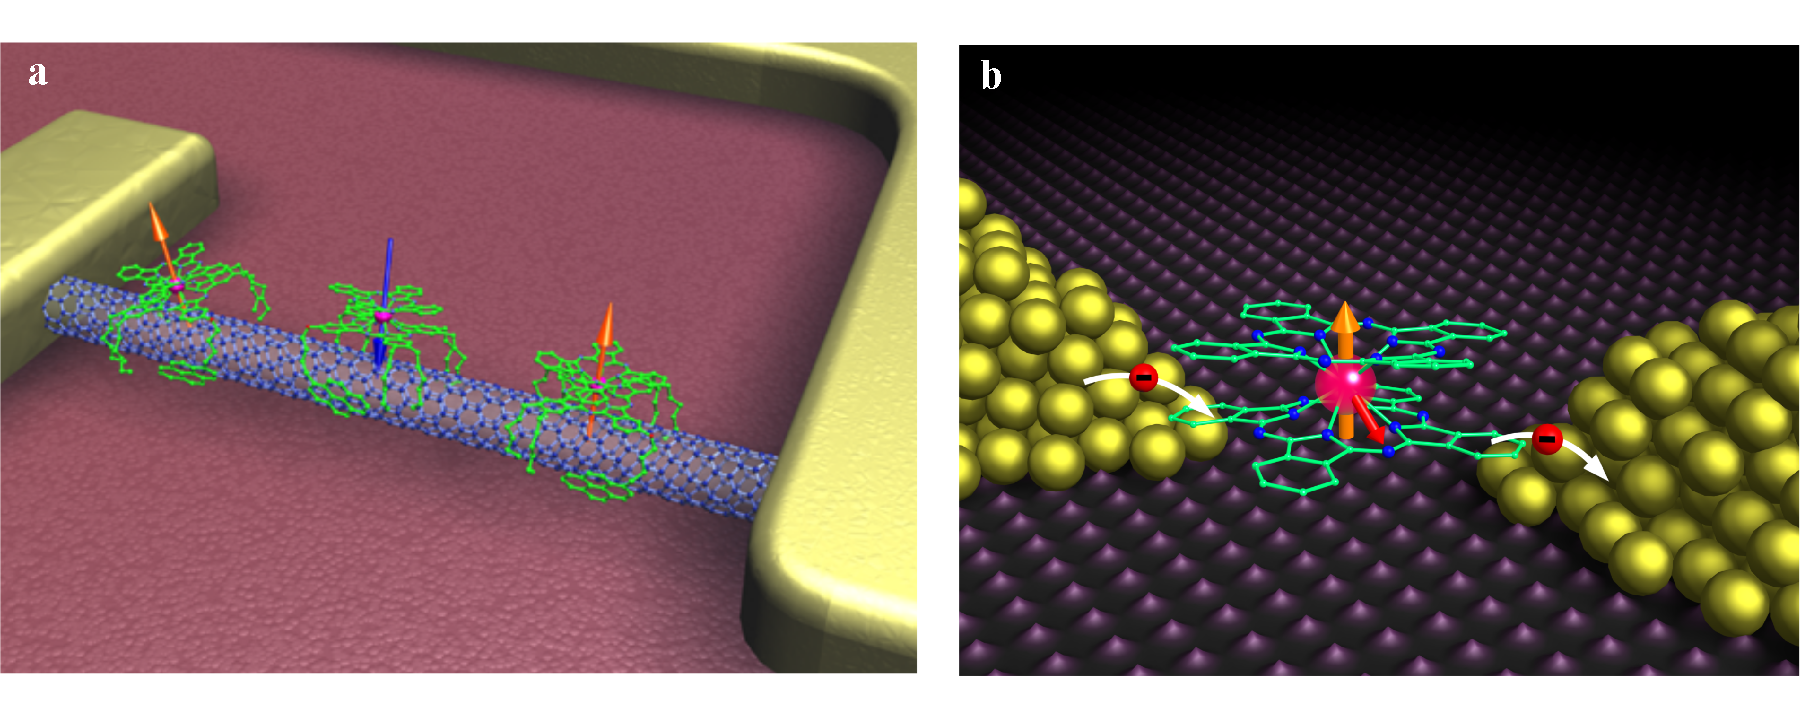
\includegraphics[scale=0.45]{Spintronique/Group2/Group2.pdf}
\caption{Vue d'artiste de la vanne de spin moléculaire~(\textbf{a}) et du transistor moléculaire~(\textbf{b}) à base de TbPc$_{2}$.}
\label{Group2}
\end{figure}

Cette analyse nous a également permis d'identifier les faiblesses de notre dispositif expérimental. Il nous fallait ajouter deux axes magnétiques pour explorer les trois directions de l'espace, mais également être capable de balayer le champ beaucoup plus rapidement : avec des vitesses de plusieurs centaines de milli-Tesla par seconde. Fort de l'expérience du groupe dans le domaine du nanomagnétisme, un dispositif mettant en jeux deux bobines de faible inductance et un système de dilution rotative a été développé rapidement au sein du laboratoire. Ce dispositif a permis d'obtenir les résultats que je vais vous présenter dans cette thèse.

La thématique des nanotubes n'est cepedant pas restée inactive, de nouveaux dispositifs ont été développés et ont donné des résultats encourageants. C'est notamment le cas de la vanne de spin obtenue par Matias Urdampilleta~\cite{Urdampilleta2011}. Dans son expérience, un tube a été relié à deux électrodes, une grille permettant de faire varier son potentiel. Un solution contenant des molécules de TbPc$_{2}$ a ensuite été déposée, puis l'échantillon a été disposé dans un frigo à dilution. Les résultats ont mis en évidence un comportement de type vanne de spin et une analyse fine des mesures a permis de déterminer que les rôles de polariseur et d'analyseur étaient joués par deux aimants moléculaires. Il s'agit là du premier dispositif de spintronique moléculaire mettant en jeux des aimants moléculaires. Il est assez amusant de constater que le premier dispositif qui a permis de mettre la spintronique sur le devant de la scène soit également la premier a être réalisé en spintronique moléculaire.
%\chapter{Fabrication d'un transistor moléculaire}

\section{Réalisation d'une grille locale}
\subsection{Quelques exemples}
\subsection{Technique de fabrication}
\subsection{Grilles obtenues à l'aide de l'ALD}


\section{Réalisation d'un nanofil}
\subsection{Lithographie optique}
\subsection{Lithographie électronique}

\section{Réalisation d'un nanogap}
\subsection{État de l'art}
\subsection{L'électromigration}

\section{Fabrication d'un transistor à molécule unique}
\subsection{Dép\^ot des molécules}
\subsection{Les trois régimes de transport}
\subsubsection{Couplage faible}
\subsubsection{Couplage intermédiaire}
\subsubsection{Couplage fort}
\chapter{Résultats expérimentaux}

\section{Le TbPc$_2$}
\subsection{Présentation}
\subsection{Origine du moment magnétique}
\subsection{Hamiltonien}
\subsection{Mesure de l'aimantation d'une assemblé}
\subsection{TbPc$_2$ et la spintronique}


\section{Mesure du retournement de l'aimantation}
\subsection{Transport à travers une boite quantique}
\subsection{Le couplage magnétisme-transport}
\subsubsection{Le couplage dipolaire}
\subsubsection{Le couplage d'échange}
\subsubsection{Le couplage magnéto-Coulomb}
\subsection{Le couplage mécanique}

\subsection{Intensité et nature de l'interaction}
\subsubsection{Amplitude des sauts de conductance}
\subsubsection{Intensité de l'interaction}

\subsection{Analyse des sauts en conductance}
\subsubsection{Méthode de détection}
\subsubsection{Interprétation physique de $\Delta g$}
\subsubsection{Choix du point de fonctionnement}
\subsubsection{Procédure d'alignement}

\subsection{Cycle d’hystérésis d'une assemblée versus une molécule isolé}
\subsubsection{A champ faible}
\subsubsection{A champ moyen}
\subsubsection{A champ fort}

\subsection{Dynamique du spin nucléaire}
\subsubsection{Temps de relaxation}
\subsubsection{Perturbations induites par la mesure}
\subsubsection{Influence de la tension de grille}
\subsubsection{Détermination de la température nucléaire}

\subsection{Perspectives}
%\chapter*{Conclusion et perspectives}
\markboth{\MakeUppercase{Conclusion et perspectives}}{\MakeUppercase{Conclusion et perspectives}}
\addcontentsline{toc}{chapter}{Conclusion et perspectives}
\setcounter{figure}{0}

Les travaux que nous venons de présenter ne sont que les premières étapes dans le développement d'une véritable spintronique à l'échelle de la molécule unique. Ils ont cependant révélé de nombreux aspects de l'interaction entre transport électronique et magnétisme moléculaire.

Ils démontrent tout d'abord la faisabilité d'une électronique moléculaire dans laquelle le magnétisme moléculaire peut être sondé. En effet, nous avons pu montrer que la conductance de notre transistor était dépendante de l'orientation du moment magnétique d'une molécule unique. Correctement utilisée, cette propriété permettrait de lire une information codée dans l'orientation de ce moment. On peut imaginer une mémoire entièrement constituée de jonctions moléculaires, et donc une grande densité de stockage.

Cette capacité de détection fait également de notre système, un détecteur d'une grande sensibilité, qui pourrait être utilisé dans le cadre du magnétisme moléculaire, pour l'investigation des propriétés quantiques des aimants moléculaires. La méthode que nous avons développé afin de reconstituer le cycle d'aimantation à l'échelle d'une molécule unique pourrait contribuer à cette étude. Notamment, l'influence de l'interaction entre l'environnement et le magnétisme moléculaire mériterait une attention particulière, même si nos résultats apportent une première information en montrant que cette dernière peut induire des transitions résonantes supplémentaires.

En outre, nous avons présenté une nouvelle technique basée sur le phénomène de QTM, permettant de mesurer, de manière non destructive, l'état d'un spin nucléaire unique, ce qui porte la sensibilité de notre système à quelques millièmes de $\mu_B$. A l'aide de celui-ci, nous avons étudié la dynamique du spin nucléaire de terbium. En particulier, nous avons mis en évidence le long temps de vie des états de spin nucléaire. La dépendance de cette dynamique vis-à-vis de l'environnement électrostatique a également été démontré même si des études plus précises seront nécessaire afin d'identifier la ou les mécanismes responsables de cette dépendance.

Cependant, de nombreux aspects de nos travaux peuvent encore être améliorés. La fabrication de nos échantillon tout d'abord qui, à ce stade, n'exploite pas encore les possibilités offertes par l'approche ``\textit{Bottom-Up}" évoquée dans le premier chapitre. En collaboration avec notre groupe, Sébastien Liatar, dans le cadre de sa thèse, a mené une étude préliminaire allant dans cette direction. La technique sur laquelle il travaillait consistait à venir attaché une molécule, par des moyens chimiques, à deux billes d'or. Il faisait ensuite, à partir de ces billes, croître des battonnet d'or de plusieurs centaines de nanomètre de longueur qu'il serait ensuite facile de contacter. Ces travaux n'ont malheureusement pas pu être menés à leur terme, et n'ont donc pas conduit à la fabrication d'un dispositif fonctionnel. Il sera donc nécessaire d'améliorer cette technique afin d'obtenir des dispositif plus aisément mais surtout, de manière reproductible.

Outre l'aspect fabrication, une bonne compréhension des phénomènes de couplage entre magnétisme moléculaire et environnement nous parait indispensable. Il faut pour cela parvenir à comprendre quels sont les mécanismes à l'origine des transitions induites que nous avons pu mesurer. Une première étude de leur position en fonction du champ transverse nous permet de penser que ces dernières sont dues à l'interaction entre la molécule aimant et un second système magnétique. Mais la nature de ce système magnétique et de l’interaction qui le couple à l'aimant moléculaire restent encore à déterminer. La travail des théoriciens à ce sujet nous apparait indispensable à la poursuite des mesures mais surtout à l'analyse de ces dernières.

De même, si le rôle important de l'environnement électrostatique, et donc du régime de transport, sur le magnétisme de notre aimant moléculaire est indiscutable, le ou les mécanismes régissant cette dépendance ne sont pas encore identifiés. Ils conduisent pourtant à une modification de la vitesse de relaxation~(cf Chap. 3), mais aussi à une suppression des transitions induites lorsque l'on se place en régime Kondo. Il reste à démontrer que ces différent phénomènes ne sont que la manifestation d'un seul et m\^eme mécanisme physique, ou bien au contraire, qu'ils sont liés à différents interactions.



\appendix
%\chapter{Les aimants moléculaires}
\section{Définition}

Un molécule, pour recevoir le qualificatif d'aimant, doit remplir deux critères. Tout d'abord, elle doit posséder un moment magnétique. Celui-ci résulte, en général, de l'interaction entre plusieurs centres magnétiques et donne lieux à un configuration où la résultante des moments magnétiques des différents centres est non nulle. 

Il faut en outre que ce moment magnétique ait une orientation préférentielle, le long de laquelle il va venir s'aligner. Les deux directions associées à cette orientation représente les deux configuration d'énergie minimale séparé par une barrière de potentiel. Afin qu'un aimant moléculaire conserve ses propriétés, il faut que l'énergie associé à l'agitation thermique soit plus faible que cette barrière. Dans le cas contraire, la température suffit à retourner aléatoirement le moment magnétique.

Certains aimants moléculaire, en plus de l'axe facile, possèdent également un plan difficile dans lequel l'énergie du moment magnétique est la plus grande. Cela donne naissance à une physique beaucoup plus riche de part l'apparition de phénomènes quantiques tels que le retournement de l'aimantation par effet tunnel~(QTM) ou bien encore la phase de Berry, que nous détaillerons dans la suite.

Malgré ces restrictions, la zoologie des aimants moléculaires est plutôt riche avec des moments magnétique allant de un à plusieurs dizaines $\mu_B$.


\section{Propriétés}
Les aimants moléculaires possèdent de nombreuses propriétés susceptibles de les rendre indispensable aux dispositifs électroniques de demain. Leur taille tout d'abord, en deçà des techniques lithographique, permettrait d'augmenter les densités de stockage, chaque molécule codant une information à travers l'orientation de son moment magnétique. Un telle application est notamment motivé par le faible taux de relaxation, de l'ordre de quelques années en dessous de $2\,K$, qui permettrait d'en faire des éléments de stockage de l'information fiable.

De plus, certains aimant moléculaires peuvent être sensible à un stimulus extérieur tels que la température, la lumières, la pression, un champ électrique ou magnétique ou bien encore un déplacement de charge. Ils peuvent ainsi osciller entre deux configurations magnétiques différentes : "haut spin" et "bas spin". Ces interrupteurs moléculaires pourraient également constituer le composant élémentaires des mémoires de demain.

Les aimants moléculaires peuvent également jouer un rôle non négligeable dans l'information quantique. Cette dernière vise à utiliser les propriétés des systèmes quantiques afin d'obtenir des algorithmes plus efficaces pour la factorisation des nombres premiers~(avec des applications dans la cryptographie notamment) ou bien encore la recherche dans les bases de données. Des phénomènes quantiques tels le QTM ou bien la phase de Berry pourrait être utilisé dans ce cadre.

Nous allons maintenant illustrer certaines de ces propriétés à travers l'exemple d'un aimant moléculaire bien connu le octanuclear fer(III) oxo-hydroxo cluster dont la formule est [Fe$_8$O$_2$(OH)$_{12}$(tacn)$_6$]$^{8+}$ ou Fe$_8$.

\section{L'exemple du Fe$_8$}

\begin{figure}
\centering \includegraphics[scale=0.45]{Annexe1/FigureFe8/FigureFe8.pdf} 
\caption{\textbf{a} : énergie en fonction du nombre quantique $m_z$. Les deux orientations $m_z=\pm 10$ sont séparées par une barrière d'énergie de hauteur $|D|S^2$~\cite{Bogani2008}. \textbf{b} : diagramme Zeeman de la molécule Fe$_8$ représentant l'énergie des différents états du système en fonction du champ magnétique. Certains croisements, comme celui marqué d'un carré, sont en fait des anti-croisements traduisant un couplage entre les états. \textbf{c} : anti-croisement représentant un couplage entre les états $m$ et $m'$. \textbf{P} est la probabilité de transition entre les états $m$ et $m'$ lorsque l'on balaie l'anti-croisement en champ magnétique. \textbf{c} : mesure de l'aimantation d'un cristal de Fe$_8$ obtenue par technique micro-squid pour différentes températures. Les anti-croisements sont visibles à travers les marches qui traduisent un renversement de l'aimantation d'un grand nombre de molécules pour des valeurs particulières du champ magnétique~(extrait de \cite{MagGoesNano}).}
\label{Fe8Zeeman}
\end{figure}


Le Fe$_8$ se compose de huit atomes de fer de degré d'oxydation III, chacun de ces atomes constituant un centre magnétique de spin 5/2. De part les différentes interactions qui les lient, ils adoptent la configuration présenté dans la Fig.\ref{Fe8Zeeman}.\textbf{b} en encart avec un moment résultant total de $S=10$, le moment magnétique des deux atomes centraux se trouvant dans la direction opposée aux six atomes latéraux.

Les propriété magnétique de ce système peuvent \^etre décrite par l'hamiltonien suivant :
\begin{eqnarray}
H =  -DS_z^2 + \frac{E}{2} ( S_+^2  + S_-^2) + g\mu_b B S_z 
\end{eqnarray}
où $D$ est le paramètre d'anisotropie axiale, $E$ est le paramètre d'anysotropie transversale, $S_z$ et la projection sur $z$ du moment magnétique et $S_+$ et $S_-$ les opérateurs création anhilation.

A champ magnétique nul, les différents états magnétiques de la molécule se trouvent de part et d'autre d'un puit de potentiel, les deux états de plus basses énergie, $m_z=\pm10$ étant séparé par une énergie $D|S|^2$ où $S$ est le moment magnétique de la molécule (cf Fig.\ref{Fe8Zeeman}.\textbf{a}). Si l'énergie associé à l'agitation thermique est telle que $k_BT \ll D|S|^2$, l'aimantation de la molécule est parfaitement définie et aligné le long de l'axe $z$. Elle peut alors avoir deux orientation : \textit{up} lorsque $m_z=+10$ et \textit{down} lorsque $m_z=-10$.

Lorsque l'on applique un champ magnétique, l'énergie associée aux différents états du système va évoluer. On peut représenter cette évolution à l'aide d'un diagramme Zeeman dans lequel on représente l'énergie de chaque niveau en fonction du champ magnétique. La Fig.\ref{Fe8Zeeman}.\textbf{b} présente le digramme Zeeman associé au Fe$_8$ pour un champ magnétique allant jusqu'à $3\,T$. Un tel diagramme comporte de nombreux croisements pour lesquels deux états du système sont dégénérés.

Cependant, la présence d'un plan difficile introduit un couplage entre certains états du système. Quand ceux-ci sont en résonance~(i.e. ont la m\^eme énergie), le couplage est maximal, ce qui se traduit dans le diagramme Zeeman par ce que l'on appelle un anti-croisement. C'est notamment le cas de l'anti-croisement repéré par un rectangle dans la Fig.\ref{Fe8Zeeman}.\textbf{b}. La Fig.\ref{Fe8Zeeman}.\textbf{c} propose une vision schématique de ce dernier où $m$ et $m'$ sont les états du système loin de la résonance, $\Delta$ désigne la séparation en énergie entre les deux états et la ligne pointillé représente le diagramme Zeeman en l'absence de plan difficile.

Lorsque l'on balaie le champ magnétique autour d'un tel anti-croisement, il y a une certaine probabilité de passer de l'état $m$ à l'état $m'$ et vice-versas. Cette probabilité est régie par la formule de Landau-Zener~\cite{Zener1932} qui dépend à la fois de la séparation minimale entre les deux niveaux~$\Delta$, ainsi que de la vitesse de balayage du champ magnétique~$\frac{dB_z}{dt}$. Cette probabilité peut s'exprimer de la façon suivante :
\begin{eqnarray}
P = 1 - \exp \left( -\frac{\pi \Delta^2}{2 \hbar g \mu_B |m-m'|\frac{dB_z}{dt}} \right)
\end{eqnarray}
ou P est la probabilité de passer de l'état $m$ à l'état $m'$. On constate tout d'abord que si la vitesse est très faible, la probabilité de passer d'un état à l'autre tend vers 1. On retrouve ici le théorème adiabatique. A l'autre bout de l'échelle, si je balaie très rapidement le champ magnétique cette probabilité tend vers zéro. Tout se passe comme si le système n'avait pas eu le temps de "sentir" l'anti-croisement.


C'est lorsque le champ magnétique balaie un anti-croisement que le phénomène de QTM pourra être observé. En effet, le système pourra alors passé d'un coté de la barrière sans avoir à fournir l'énergie correspondante. Autrement dit, le renversement va se faire par effet tunnel à travers la barrière le potentiel, d'où le nom de renversement de l'aimantation par effet tunnel~(Qantum Tunneling of the Magnetization ou QTM en anglais).

Ce phénomène quantique peut être mise en évidence par une mesure de l'aimantation d'une assemblé de molécule. Une telle mesure consiste à relever l'aimantation d'un cristal moléculaire en fonction du champ magnétique. L'aimantation du cristal est d'abord amenée à saturation par l'application d'un fort champ magnétique. Celui-ci est ensuite balayé jusqu'à obtenir la saturation du cristal dans la direction opposée. Lorsque l'aimantation des molécules composant le cristal se retourne, elles modifient les lignes de champ environnante. De telle variation peuvent \^etre mesuré par une technique de micro-SQUID. La Fig.\ref{Fe8Zeeman}.\textbf{d} présente la mesure de l'aimantation d'un cristal de Fe$_8$ pour différentes températures et pour une vitesse de balayage de $14\,mT.s^{-1}$.

La courbe montre une série de marches qui sont d\^ues au retournement par QTM. Chacune d'elles correspond à un anti-croisement sur lequel l'aimantation à une probabilité élevée de transiter. Lorsque l'on diminue la température, le taux de retournement diminue car les transitions assistées thermiquement diminuent. Cette courbe devient indépendante de la température au dessous de 400\,mK et on observe les transitions correspondantes aux niveaux de plus basse énergie. 

%\input{Annexe2/Annexe2.tex}
%\chapter{\'Equation pilote}
Une manière plus précise de poser le problème du courant, comparativement à celle présentée dans l'Annexe A, est d'utiliser la méthode des équations pilotes. On peut diviser la procedure à suivre en trois étapes. La première étape consiste à déterminer les différents états possibles de l'\^ilot, de leur attribuer à chacun une probabilité et de mettre en évidence ensuite les différentes relations de transition d'un état à l'autre. Une fois ceci fait, il faut déterminer les paramètres physiques permettant le passage d'un état à l'autre en exprimant les taux de transition que l'on notera $\Gamma$. Enfin, à partir des taux de transitions et des différentes probabilités d'état, on peut exprimer le courant circulant dans le système.

\section{Les différents états du système et leur probabilités}
On suppose ici que l'état de charge de l'\^ilot est soit $N=0$ soit $N=1$. Si l'on tient compte de l'état de spin de l'électron, l'on peut associer à chacun de ces états une probabilité (P$_0$,P$_-$ et P$_+$ respectivement) en attribuant un $+$ pour l'état spin up et $-$ à l'état de spin down. On peut facilement établir entre ces probabilité les relations suivantes:

\begin{eqnarray}
\frac{dP_0}{dt} &=& \Gamma_{+ \rightarrow 0}P_+ + \Gamma_{- \rightarrow 0}P_-  -(\Gamma_{0 \rightarrow +}P_0 + \Gamma_{0 \rightarrow -}P_0) \nonumber \\
\frac{dP_\pm}{dt} &=& \Gamma_{0 \rightarrow \pm}P_0 - \Gamma_{\pm \rightarrow 0}P_\pm \nonumber
\end{eqnarray}
ou $\Gamma_{\alpha \rightarrow \beta}$ est le taux de transition de l'état $\alpha$ à l'état $\beta$. En régime permanent, les différentes probabilités ne dépendent plus du temps et on peut donc en déduire les relations suivantes :
\begin{eqnarray}
P_0 &=& \frac{\Gamma_{+ \rightarrow 0}P_{+} + \Gamma_{- \rightarrow 0}P_{-}}{\Gamma_{0 \rightarrow -} + \Gamma_{0 \rightarrow +} }\\
P_{\pm} &=& \frac{\Gamma_{\pm \rightarrow 0}}{\Gamma_{0 \rightarrow \pm}}P_0 
\end{eqnarray}

Ce qui peut être reformuler de la façon suivante:
\begin{eqnarray}
P_0 &=& \frac{1}{1 + \frac{\Gamma_{0 \rightarrow +}}{\Gamma_{+ \rightarrow 0}} + \frac{\Gamma_{0 \rightarrow -}}{\Gamma_{- \rightarrow 0}}} \\
P_{\pm} &=& \frac{\Gamma_{\pm \rightarrow 0}}{\Gamma_{0 \rightarrow \pm}}P_0 
\end{eqnarray}


Il nous faut maintenant exprimer les taux de transition $\Gamma_{0 \rightarrow \pm}$ et $\Gamma_{\pm \rightarrow 0}$ en fonction des paramètres du système. 

\section{Détermination des taux de transfert}
Nous allons tout d'abord nous intéresser au taux de transfert $\Gamma_{0 \rightarrow \pm}$ car le raisonnement à faire est très proche de celui effectué dans l'Annexe A dans le cadre des potentiels chimiques. 

Comme nous l'avons déjà montré plus haut, il y a deux façons de charger l'\^ilot : par la source ou par le drain. On a donc :
\begin{eqnarray}
\Gamma_{0 \rightarrow \pm} = \Gamma_{0 \rightarrow \pm}^s + \Gamma_{0 \rightarrow \pm}^d
\end{eqnarray}
où nous avons diviser le taux de transfert en un taux de transfert source et un taux de transfert drain. Il s'agit donc de trouver dans la source (ou le drain) un électron dont le potentiel chimique correspond à la transition $0\rightarrow \pm$. Nous noterons le potentiel chimique associé à cette transition $\mu_{\pm}$ dans la suite. 

Son expression peut facilement se déduire de l'Equ.\ref{pot_chim} et exprimer sous la forme suivante :
\begin{eqnarray}
\mu_{\pm} = \frac{1}{2}E_c - \frac{E_c}{|e|}(C_gV_g + C_sV_s + C_dV_d)~ \pm \underbrace{ \frac{1}{2}g \mu_B B}_{\text{terme Zeeman}}
\end{eqnarray}
ou  $\mu_B$ et le magnéton de Bohr, $g$ est le facteur de Landé et $B$ est le champ magnétique appliqué au système.

Si on se réfère au paragraphe précédent, le probabilité de trouver un électron dans la source ou dans le drain dont le potentiel chimique est égal à $\mu_{\pm}$ est donnée par :
\begin{eqnarray}
p_i(\mu_\pm) = \frac{1}{1 + \exp{(\frac{\mu_\pm - eV_i}{k_bT})}}
\end{eqnarray}
ou $i=source/drain$. 

Du fait de la présence d'une barrière tunnel entre la source ou le drain et l'\^ilot, cette probabilité doit être pondérée par un terme relatif au couplage que l'on notera $\gamma_i$ ou $i=source/drain$.
On peut donc écrire:
\begin{eqnarray}
\Gamma_{0 \rightarrow \pm} =& \Gamma_{0 \rightarrow \pm}^s + \Gamma_{0 \rightarrow \pm}^d  \nonumber \\
 =& \gamma_s p_s(\mu_\pm) + \gamma_d p_d(\mu_\pm)
\end{eqnarray}

Par un raisonnement identique on peut déterminer $\Gamma_{\pm \rightarrow 0}$. La seule modification au raisonnement est qu'il faut cette fois-ci qu'un état soit libre dans la source ou dans le drain ce qui correspond à une probabilité de :
\begin{eqnarray}
1 - p_i(\mu_\pm) &=& 1 - \frac{1}{1 + \exp{(\frac{\mu_\pm - eV_i}{k_bT})}} \nonumber \\
 &=& \frac{\exp{(\frac{\mu_\pm - eV_i}{k_bT})}}{1 + \exp{(\frac{\mu_\pm - eV_i}{k_bT})}}
\end{eqnarray}
ou $i=source/drain$.
En effectuant cette subtitution, on trouve facilement :
\begin{eqnarray}
\Gamma_{\pm \rightarrow 0} =& \Gamma_{\pm \rightarrow 0}^s + \Gamma_{\pm \rightarrow 0}^d  \nonumber \\
 =& \gamma_s \{1 - p_s(\mu_\pm)\} + \gamma_d \{1-p_d(\mu_\pm)\}
\end{eqnarray}
Nous avons désormais tous les éléments pour exprimer le courant circulant dans notre système. C'est cette dernière étape que nous allons aborder maintenant.
\section{Détermination du courant}
De part la loi de conservation, on peut calculer indifféremment le courant au niveau de la source ou au niveau du drain. Si l'on se place du c\^oté de la source, on peut voir que le courant est composé d'une composante positive de part les électrons qui quittent la source pour l'\^ilot, et une composante négative  de part les électrons de l'\^ilot qui se déchargent dans la source. Ces deux composantes peuvent s'exprimer de la façon suivante:
\begin{eqnarray}
I = |e| \gamma_s [(\Gamma_{0 \rightarrow +}^s + \Gamma_{0 \rightarrow -}^s) P_0 - \{ \Gamma_{+ \rightarrow 0}^s P_{+} + \Gamma_{- \rightarrow 0}^s P_{-}  \}]
\end{eqnarray}


On peut voir dans la Fig. \ref{SimulatedCoulombMap} le courant correspondant ainsi que sa dérivée relative à la tension $V_{ds}$ dans le plan ($V_g$,$V_{ds}$). Le tracé a été fait sans champ magnétique appliqué.


\begin{figure}
\begin{center}
\includegraphics[scale=0.5]{Annexe3/figure1/figure4.pdf} 
\caption{Courant correspant à un état de charge (0,1) dans le plan ($V_g$,$V_{ds}$) sans champ magnétique}
\label{SimulatedCoulombMap}
\end{center}
\end{figure}

\subsubsection{Quelques remarques}
Il convient toutefois de faire quelques remarques sur cette méthode des équations pilotes. Tout d'abord, nous n'avons pas tenu compte des relaxations à l'intérieur de l'\^ilot. Pour inclure de tel phénomène, il faudrait introduire des taux de transfert du type $\Gamma_{\pm \rightarrow \mp}$. De plus, afin que dans le cas d'un système isolé, l'on retrouve une distribution de type Bolzman, il faudra s'assurer que ces deux taux de transfert obéissent à la relation suivante :
\begin{eqnarray}
\frac{\Gamma_{+ \rightarrow -}}{\Gamma_{- \rightarrow +}} = \exp(\frac{\mu_{+}- \mu_{-}}{k_bT}) \nonumber
\end{eqnarray}

Deuxième remarque, l'élargissement des niveau au sein de l'\^ilot n'est pas pris en compte. Dans le régime fortement bloqué que nous avons choisi comme modèle ici, cette hypothèse est raisonnable. 

Troisième remarque, la méthode de l'équation pilote n'est valable que dans le cas d’événements tunnel des électrons indépendants les uns de autres. Cette méthode ne peut donc pas \^etre utiliser dans le traitement du cotunneling.


%\chapter{Article Phys. Rev. B : Cotunneling through a magnetic single-molecule transistor based on N@C$_{60}$}
%\includepdf[pages = {1-4}]{Articles/prb_83_081407.pdf}


%\chapter{Article Nature : Electronic read-out of a single nuclear spin using a
%molecular spin transistor}
%\includepdf[pages = {1-4}]{Articles/nature11341.pdf}

\bibliographystyle{unsrt}
\bibliography{citations}

\end{document}
